% Extremal equal-spin EGB black holes built directly at T = 0:
% reproduction of arXiv:2303.12471 (equal spins) and the extremal mass shift.
% Every number is a macro from numbers.tex (make_report_numbers.py).
% Build: cd work/kkr-extremal/report && tectonic -X compile report.tex
\documentclass[11pt,a4paper]{article}
\usepackage[T1]{fontenc}
\usepackage{lmodern}
\usepackage[margin=2.4cm]{geometry}
\usepackage{amsmath,amssymb}
\usepackage{booktabs}
\usepackage{graphicx}
\usepackage{xcolor}
\usepackage[colorlinks=true,allcolors=blue!55!black]{hyperref}
% generated by make_report_numbers.py; do not edit
\newcommand{\Rgammamin}{1.773}
\newcommand{\Rgammaminy}{0.029}
\newcommand{\Rgammaymax}{36.3}
\newcommand{\Rgammacrosstwo}{0.71}
\newcommand{\Rgammacrossthree}{4.51}
\newcommand{\Rgammasmally}{0.0009}
\newcommand{\Rdigitworst}{3.7\times10^{-4}}
\newcommand{\Rconvaalpha}{0.05}
\newcommand{\Rconvamu}{2.3280174}
\newcommand{\Rconvamums}{2.3280172}
\newcommand{\Rconvay}{0.0568894}
\newcommand{\Rconvayms}{0.0568895}
\newcommand{\Rconvbalpha}{0.2}
\newcommand{\Rconvbmu}{2.5319363}
\newcommand{\Rconvbmums}{2.5319363}
\newcommand{\Rconvby}{0.2290601}
\newcommand{\Rconvbyms}{0.2290603}
\newcommand{\Rconvcalpha}{0.5}
\newcommand{\Rconvcmu}{2.8885348}
\newcommand{\Rconvcmums}{2.8885349}
\newcommand{\Rconvcy}{0.5112438}
\newcommand{\Rconvcyms}{0.5112439}
\newcommand{\Rbranchpoints}{268}
\newcommand{\Ralphamax}{3.118}
\newcommand{\Rymax}{2.443}
\newcommand{\Rxmax}{0.863}
\newcommand{\Rjlast}{0.189}
\newcommand{\Rnmaxbranch}{312}
\newcommand{\Rconstraintworst}{7.3\times10^{-5}}
\newcommand{\Rdmuworst}{7.4\times10^{-5}}
\newcommand{\Rdslopeworst}{8.7\times10^{-3}}
\newcommand{\Rcleanrows}{183}
\newcommand{\Rfirstlawworst}{3.7\times10^{-6}}
\newcommand{\Rfirstlawmedian}{7.2\times10^{-8}}
\newcommand{\Rsmarrworst}{2.8\times10^{-5}}
\newcommand{\Rsmarrmedian}{5.4\times10^{-7}}
\newcommand{\Romegaidclean}{5.2\times10^{-5}}
\newcommand{\Rvonedev}{3.3\times10^{-6}}
\newcommand{\RhHdev}{2.4\times10^{-7}}
\newcommand{\Rsigmanhdev}{3.8\times10^{-4}}
\newcommand{\Romegaiddev}{1.2\times10^{-2}}
\newcommand{\Rslopemin}{1.0710}
\newcommand{\Rslopeminy}{0.195}
\newcommand{\Rslopelast}{2.1775}
\newcommand{\Rmugrowth}{203}
\newcommand{\RkkraHdev}{6.5\times10^{-4}}
\newcommand{\RkkraHdevj}{1.2\times10^{-3}}
\newcommand{\Rkkrsdev}{1.4\times10^{-3}}
\newcommand{\Rkkrsdevj}{2.6\times10^{-3}}
\newcommand{\Rpolishedcouplings}{12}
\newcommand{\Rdmuworstms}{6.2\times10^{-6}}
\newcommand{\Rdpsiworstms}{1.9\times10^{-5}}
\newcommand{\Rdyworstms}{3.4\times10^{-7}}
\newcommand{\Rpsiratioworst}{1.8\times10^{-3}}
\newcommand{\Rcomparisontable}{%
  $0.005$ & $0.004790$ & $2.2115781$ & $9.9\times10^{-7}$ & $2.2115792$ & $1.3\times10^{-3}$ & $2.990940$ & $5.4\times10^{-6}$ & $2.990943$ & $1.1\times10^{-1}$ \\
  $0.01$ & $0.009845$ & $2.2262777$ & $7.1\times10^{-7}$ & $2.2262788$ & $7.7\times10^{-4}$ & $2.824561$ & $3.5\times10^{-6}$ & $2.824558$ & $8.8\times10^{-2}$ \\
  $0.02$ & $0.020720$ & $2.2550577$ & $1.2\times10^{-6}$ & $2.2550579$ & $1.6\times10^{-3}$ & $2.472846$ & $4.4\times10^{-6}$ & $2.472827$ & $1.6\times10^{-1}$ \\
  $0.035$ & $0.038427$ & $2.2944442$ & $9.4\times10^{-7}$ & $2.2944380$ & $8.4\times10^{-4}$ & $2.000655$ & $2.0\times10^{-6}$ & $2.000660$ & $9.0\times10^{-2}$ \\
  $0.05$ & $0.056889$ & $2.3280166$ & $8.0\times10^{-7}$ & $2.3280172$ & $5.7\times10^{-6}$ & $1.659079$ & $9.0\times10^{-7}$ & $1.659080$ & $8.6\times10^{-3}$ \\
  $0.075$ & $0.087750$ & $2.3734822$ & $2.2\times10^{-7}$ & $2.3734823$ & $9.1\times10^{-6}$ & $1.325970$ & $9.2\times10^{-8}$ & $1.325970$ & $2.4\times10^{-3}$ \\
  $0.1$ & $0.117873$ & $2.4107272$ & $1.5\times10^{-6}$ & $2.4107287$ & $3.7\times10^{-5}$ & $1.166215$ & $1.9\times10^{-8}$ & $1.166214$ & $8.3\times10^{-4}$ \\
  $0.15$ & $0.175201$ & $2.4739927$ & $4.7\times10^{-7}$ & $2.4739932$ & $1.1\times10^{-5}$ & $1.071493$ & $1.3\times10^{-7}$ & $1.071492$ & $2.3\times10^{-3}$ \\
  $0.2$ & $0.229060$ & $2.5319360$ & $4.3\times10^{-7}$ & $2.5319363$ & $8.8\times10^{-6}$ & $1.090071$ & $1.5\times10^{-7}$ & $1.090070$ & $2.8\times10^{-3}$ \\
  $0.3$ & $0.329212$ & $2.6465810$ & $1.2\times10^{-6}$ & $2.6465821$ & $4.5\times10^{-6}$ & $1.207815$ & $4.1\times10^{-7}$ & $1.207813$ & $2.1\times10^{-3}$ \\
  $0.4$ & $0.422511$ & $2.7651786$ & $1.2\times10^{-6}$ & $2.7651797$ & $4.6\times10^{-6}$ & $1.333843$ & $4.3\times10^{-7}$ & $1.333842$ & $2.7\times10^{-3}$ \\
  $0.5$ & $0.511244$ & $2.8885340$ & $8.0\times10^{-7}$ & $2.8885349$ & $1.1\times10^{-6}$ & $1.444398$ & $3.5\times10^{-7}$ & $1.444398$ & $6.2\times10^{-4}$ \\
}
\newcommand{\Rgcplateau}{38}

\newcommand{\ext}{\mathrm{ext}}
\newcommand{\GB}{\mathrm{GB}}

\title{Extremal equal-spin Einstein--Gauss--Bonnet black holes at $T=0$:\\
reproduction of arXiv:2303.12471 and the extremal mass shift}
\author{}
\date{\today}

\begin{document}
\maketitle

\section{What was done}

\begin{enumerate}
\item The equal-spin, asymptotically flat part of arXiv:2303.12471
(Kleihaus, Kunz, Radu; KKR below) was reproduced: the near-horizon closed forms
of its section~3.2 and the extremal boundary of the domain of existence in the
left panels of its fig.~1, against curves extracted from the vector EPS files of
the arXiv source.
\item A spectral solver was built for the \emph{extremal} solutions themselves, in
KKR's gauge, with the two zero modes of that gauge identified and fixed. It gives
$M_\ext(J,\alpha)$, $\mu(y)=M_\ext/J^{2/3}$ and the slope
$\partial M_\ext/\partial\alpha|_J=\mu'(y)$ directly at $T=0$, the latter by
implicit differentiation of the discrete system.
\item The result was compared with the manuscript's $T\to0$ extrapolation of
non-extremal solutions (\texttt{results/egb-extremality.json}).
\item The perturbations of the extremal throat were analysed: the horizon is not
smooth at finite coupling.
\end{enumerate}

\noindent Units: $r_H=1$, i.e.\ $g_H=1$ for the round part of the horizon metric, as in
the manuscript; $J$ is the angular momentum in \emph{each} plane;
$y=\alpha/J^{2/3}$, $x=3\pi\alpha/(4M)$, $j=(3/2)^{3/2}\sqrt\pi J/M^{3/2}$.

\section{Field equations and checks}

The reduced Lagrangian of arXiv:1010.0860 (as transcribed and validated in the
project with $g=r^2$) was used with the squashing function $g$ left free, since
the extremal gauge needs it. Its Euler--Lagrange equations for
$(b,f,g,h,w)$ agree with $-\sqrt{bh/f}\,g\,(G+\alpha H)^{\mu\nu}\partial
g_{\mu\nu}/\partial v$ from the independent tensor evaluator on generic,
non-solution jets of all five functions (\texttt{derive.py}).

\section{The near-horizon geometry and a non-smooth horizon}

On $b=v_1\rho^2$, $g^{\rho\rho}=\rho^2/v_1$, $g=G_0$, $h=H_0$, $w'=w_1$ the
equations reduce to three algebraic relations. Their solution reproduces KKR's
eqs.~(at7)--(at9) to round-off on 60 points of their $v_3$ parametrisation, with
one convention difference: the ``$J$'' of their eq.~(at9) is $J_1+J_2$, twice the
per-plane $J$ of their asymptotic formula. At $\alpha=0$ it is the extremal
Myers--Perry throat, $S=2\pi J$.

Linearising about the throat with $\delta\propto\rho^\gamma$ (gauge
$g^{\rho\rho}$ fixed) gives exponents in AdS$_2$ pairs $(\gamma,-1-\gamma)$. At
$\alpha=0$ they are the integers $\{-3,-2,0,0,1,2\}$; at finite coupling the
growing exponent $2$ becomes a non-integer $\gamma(y)$
(fig.~\ref{fig:gamma}). It falls to $\Rgammamin$ at $y=\Rgammaminy$, returns
through $2$ at $y=\Rgammacrosstwo$ and through $3$ at $y=\Rgammacrossthree$
(scanned up to $y=\Rgammaymax$). A generic extremal solution excites this mode, so
for $\gamma<2$ its metric functions are $C^1$ but not $C^2$ in $\rho$ at the
horizon (a statement about the metric functions; curvature in a parallelly
propagated frame was not computed). This is, as far as recalled and not re-read
here, the equal-spin Gauss--Bonnet counterpart of the non-smooth extremal horizons
reported for Kerr with higher-derivative corrections (arXiv:2303.07358). It also
means that KKR's ``approximate form of the solutions as a power series in $r$'' at
the horizon (their $r^2\propto\rho$) cannot be exact: the expansion needs
$r^{2\gamma}$ terms.

\emph{How this was checked.} The exponents come from the linear analysis, which
is integer at $\alpha=0$ and pairs correctly at every coupling. In the full
solutions the effect shows up indirectly: in a representation where the mass is
read from a second derivative at infinity, it converges only algebraically, while
an analytic solution converges geometrically; and the constraint violation and the
resolution differences peak next to the horizon. A direct fit of the Chebyshev
tail of the production solutions does \emph{not} resolve the exponent, because
the tail reaches the round-off plateau by $n\approx\Rgcplateau$, before an algebraic
decay $n^{-(4\gamma+1)}$ becomes visible.

\begin{figure}[t]
\centering
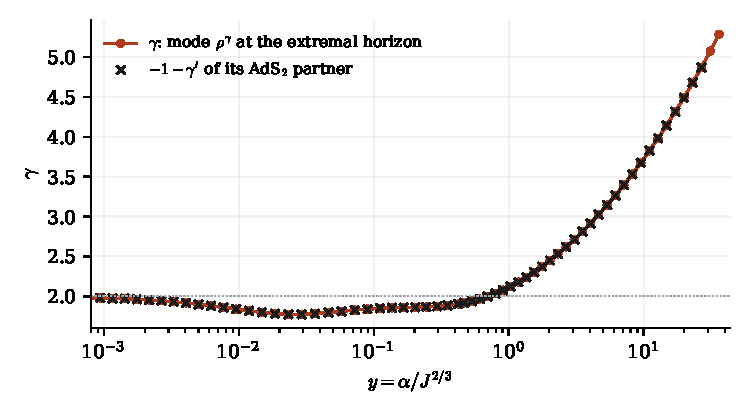
\includegraphics[width=.72\textwidth]{../figures/fig3-exponent.pdf}
\caption{Exponent of the growing perturbation of the extremal throat,
$\delta\propto\rho^\gamma$, and of its AdS$_2$ partner $-1-\gamma'$; integer
($\gamma=2$) only at $y=0$ and at isolated couplings.}
\label{fig:gamma}
\end{figure}

\section{The extremal solver}

\paragraph{Gauge.} KKR's ansatz with $a=1$ and $P_i=e^{2F_i}$:
$b=P_1r^4/(u^2+1)$, $g^{rr}=P_1^{-1}r^2/u$, $g=P_2u$, $h=P_2P_3u(1+u^{-2})$,
$w=\sqrt2/(u^2+1)+W$, $u=r^2+1$. The product $b\,g^{rr}$ is fixed. This is what
makes the extremal problem well posed numerically. In the gauge $g=r^2$, with the
double zero factored out of $b$ and $f$, nearby non-extremal solutions are almost
representable by polynomials (both $b$ and $f$ pick up the same $1/x$ factor), and
the collocation matrix became singular as $N$ grew. That route was abandoned.

\paragraph{Zero modes.} With $a$ and $\alpha$ fixed the gauge still leaves two
exact zero modes, identified from smooth, resolution-independent null vectors of
the Jacobian: (i) the physical size of the black hole relative to $a$, and (ii)
the residual radial gauge $r\to r+c\sqrt{b\,g^{rr}}$, which is $\propto r^3$ at
the horizon and a constant shift at infinity. They are fixed by $g_H=P_2(0)=1$
and by the absence of a $1/r$ term in $P_2$.

\paragraph{Discretisation.} Chebyshev collocation in $s=r/(1+r)$, in which the
residual-gauge term $r^3$ and the asymptotic tails are smooth and only
$r^{2\gamma}$ remains singular. The unknowns are $Q_i$ with
$P_i=1+(1-s)^2Q_i$ and $W=(1-s)^2Q_4$. This builds in asymptotic flatness and the
gauge condition, and makes the mass a value at infinity,
$M=\tfrac{3\pi}{4}(1-c_t)$ with $c_t=Q_1(1)/2$. In the $P$ representation $c_t$
was $P_1''(1)/4$, weighted by $k^4$ in the Chebyshev tail and converging only
algebraically. $J$ is the conserved momentum of $w$, $J=-\tfrac{\pi}{16}\partial
L/\partial w'$, evaluated in the interior. At $s=0$ the $E_{P_i}$ rows vanish
identically and are replaced by $\mathrm dP_i/\mathrm ds=0$; at $s=1$ all four
equations vanish identically in this representation and are collocated at a point
between the last two nodes. The residuals were generated symbolically in three
expanded forms (near each end and in between) to avoid cancellation. The Jacobian
is assembled by the chain rule and agrees with a dense complex-step Jacobian to
round-off.

\paragraph{Validation.} At $\alpha=0$ Newton returns extremal Myers--Perry with
$M=3\pi/4$, $J=\pi\sqrt2/4$, $\Omega_H=1/\sqrt2$, $S=2\pi J$, $j=1$,
$a_H=s=\tfrac12$. Over the branch the Hamiltonian constraint, which is not
imposed, stays below $\Rconstraintworst$. The horizon data agree with the
near-horizon solution at the same $\alpha/g_H$: $P_1(0)/4=v_1$ to $\Rvonedev$,
$h_H=H_0$ to $\RhHdev$. Two identities are evaluated, not imposed. Over the $\Rcleanrows$ branch points whose two resolutions agree to
$10^{-5}$ in $\mu$ and $\mu'$: the first law at $T=0$ along the branch,
$\Psi=M_\alpha-2\Omega_HJ_\alpha$, agrees with the implicitly differentiated slope
to $\Rfirstlawworst$ (median $\Rfirstlawmedian$); Smarr at $T=0$,
$\Psi=(M-3\Omega_HJ)/\alpha$, to $\Rsmarrworst$ (median $\Rsmarrmedian$) for
$\alpha\ge0.05$, since it divides by $\alpha$; and the identity
$3\omega=\mu-y\mu'$ of the manuscript holds to $\Romegaidclean$. The acceptance threshold on the constraint was $10^{-6}$ up to $\alpha\approx0.76$,
$10^{-5}$ up to $\alpha\approx2.29$ and $10^{-4}$ beyond; the comparison with the
manuscript (table~\ref{tab:compare}) uses separate high-resolution solutions, not
the branch. Spurious roots of the discrete system exist (non-decaying
Chebyshev tails, constraint $\sim10^{-3}$) and are rejected by those two
diagnostics. At larger coupling Newton needs a tangent predictor to stay on the
physical root.

\section{Reproduction of fig.~1 of arXiv:2303.12471}

The vector paths of the six \texttt{*-MP2.eps} panels were mapped to data
coordinates through each plot's own tick labels. Against the closed-form static
curves the calibration is good to $\Rdigitworst$, about one device unit. On the
range we construct ($x\le\Rxmax$), our extremal branch agrees with KKR's extremal
curve to $\RkkraHdev$ in $a_H(x)$ and $\Rkkrsdev$ in $s(x)$, and to $\RkkraHdevj$
and $\Rkkrsdevj$ in the insets against $j$ (fig.~\ref{fig:fig1}). The boundaries
$j\le1$ and $x<1$ hold; $j$ falls to $\Rjlast$ at the largest coupling reached.
KKR continue to $x\approx0.92$ and draw a hand extrapolation to the singular static
point $(x,j)=(1,0)$. Our branch stops at $\alpha=\Ralphamax$ ($y=\Rymax$,
$x=\Rxmax$): beyond it the constraint violation, concentrated next to the
horizon, exceeds $10^{-4}$ even at $N=\Rnmaxbranch$, and the round-off floor of the
residual rules out higher $N$. Going further needs a coordinate that resolves the
horizon region better, or extended precision, not more continuation.

\begin{figure}[p]
\centering
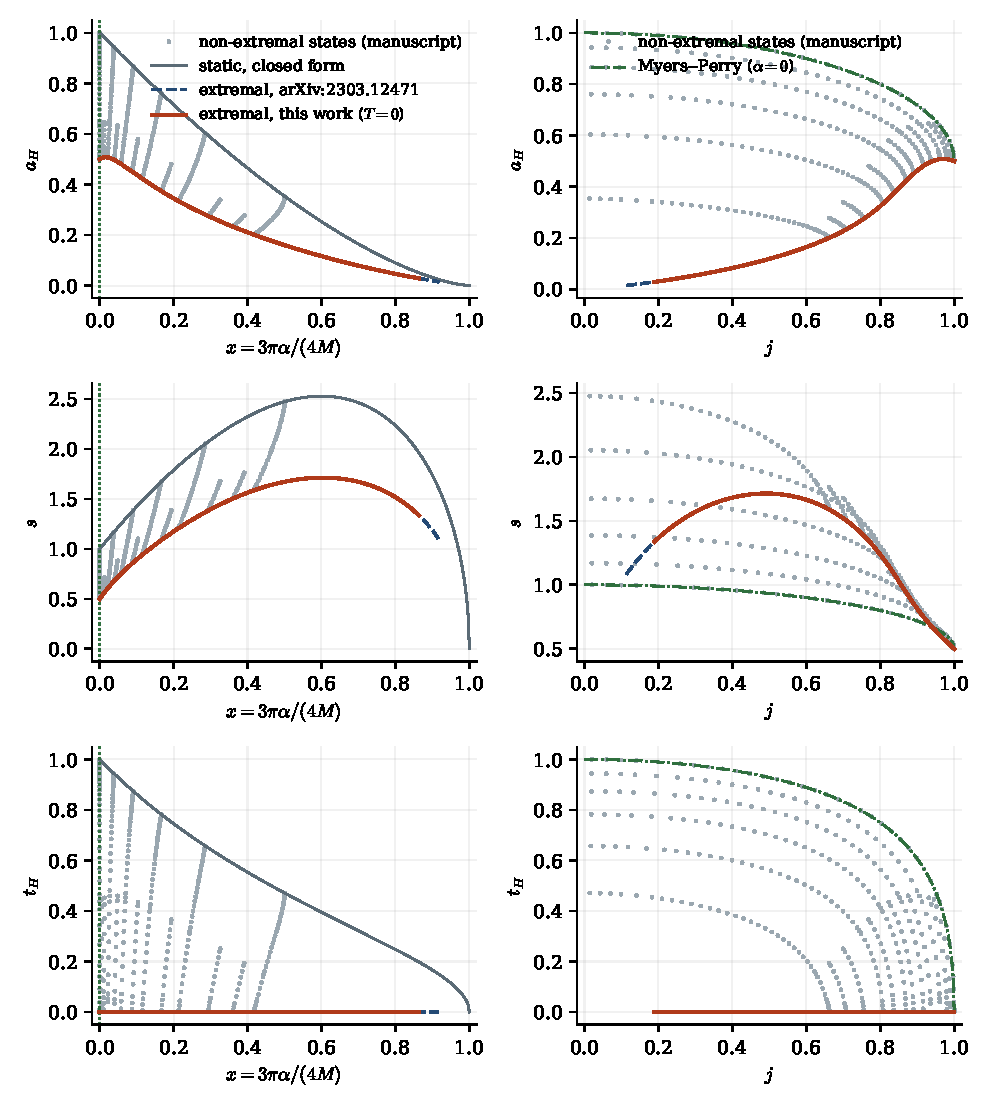
\includegraphics[width=\textwidth]{../figures/fig1-reproduction.pdf}
\caption{Left panels of fig.~1 of arXiv:2303.12471. Left column against
$x=3\pi\alpha/(4M)$, right column (their insets) against $j$. Grey: non-extremal
states of the manuscript; solid grey-blue: static family (closed form);
dash-dotted green: Myers--Perry; dashed blue: KKR's extremal curves, from their
EPS; solid red: extremal solutions constructed here at $T=0$.}
\label{fig:fig1}
\end{figure}

\section{The extremal mass shift}

Fig.~\ref{fig:shift} shows $\mu(y)$ and $\mu'(y)$ on the branch. The slope starts
at $\pi$, falls to $\Rslopemin$ at $y=\Rslopeminy$ and rises again, reaching
$\Rslopelast$ at the end of the branch; $\mu$ grows by $\Rmugrowth\%$ over the
range. Table~\ref{tab:compare} compares the extremal solutions, computed at
$N=64,96,128$ at each of the manuscript's $\Rpolishedcouplings$ finite couplings,
with the manuscript's $T\to0$ extrapolations at the same $\alpha$. Across them
$y$ agrees to $\Rdyworstms$ and $\mu$ to $\Rdmuworstms$. The manuscript's
$\Psi_\ext$ agrees with the directly computed slope to $\Rdpsiworstms$, at most
$\Rpsiratioworst$ of its own fit-sensitivity envelope. The extrapolated central
values are therefore far more accurate than the envelope suggests. Where the two
differ in $\mu$ by more than the manuscript's three-fit spread, the difference is
still at the $10^{-6}$ level.

\begin{table}[t]
\centering\footnotesize
\setlength{\tabcolsep}{2.6pt}
\begin{tabular}{@{}cccccccccc@{}}
\toprule
$\alpha$ & $y$ & $\mu$ (this work) & res. & $\mu$ (ms) & spread &
$\mu'$ (this work) & res. & $\Psi_\ext$ (ms) & envelope\\
\midrule
\Rcomparisontable
\bottomrule
\end{tabular}
\caption{Extremal solutions at $T=0$ against the manuscript's $T\to0$
extrapolation (ms). ``res.'' is the larger of the differences between $N=128$
and $96$ and between $96$ and $64$: a resolution difference, not a bound.
``spread'' is the manuscript's three-fit degree spread of $\mu$, ``envelope''
its twenty-fit sensitivity of $\Psi_\ext$.}
\label{tab:compare}
\end{table}

\begin{figure}[t]
\centering
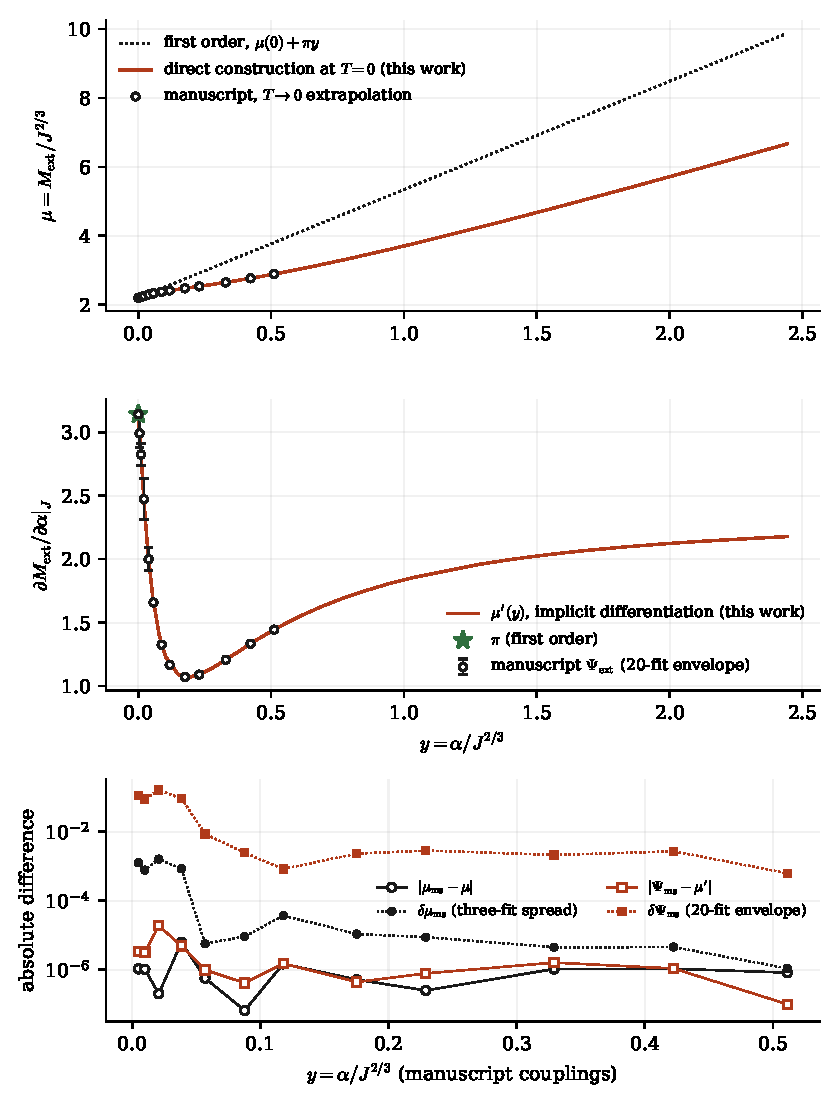
\includegraphics[width=.8\textwidth]{../figures/fig2-mass-shift.pdf}
\caption{Top: $\mu(y)$ from the extremal solutions (line) and the manuscript's
extrapolations (circles); dotted: first order. Middle: slope by implicit
differentiation (line) and the manuscript's $\Psi_\ext$ with its envelope.
Bottom: differences in units of the manuscript's own spreads.}
\label{fig:shift}
\end{figure}

\section{What was not checked}

\begin{itemize}
\item No independent check of the field equations beyond the tensor route on
generic jets and the closed forms; the near-horizon identification is KKR's.
\item The resolution differences are differences, not error bounds. The round-off
floor of the residual grows with $N$ and limits the attainable accuracy to about
$10^{-7}$--$10^{-6}$ in $\mu$; above $N\approx100$ more resolution does not help.
\item The non-smooth exponent is established by the linear analysis; the full
solutions are consistent with it but do not measure it independently.
\item The branch does not reach $x\approx0.92$ as KKR do; the endpoint conjecture
$(x,j)\to(1,0)$ is not tested.
\item The digitised curves of KKR are compared on the range we construct; no
statement is made about their accuracy beyond the figure.
\item The interior of the domain of existence is shown only through the
manuscript's states ($\alpha\le\tfrac12$); KKR's interior scan was not repeated.
\end{itemize}

\section{Run receipt}
\begin{itemize}\itemsep0pt
\item date of this build: 2026-10-07; directory \texttt{work/kkr-extremal}
\item environment: Python 3.10.12, NumPy 2.2.6, SciPy 1.15.3, SymPy 1.14.0 (project \texttt{.venv})
\item \texttt{eps\_digitise.py; kkr\_curves.py} $\to$ digitised.json, kkr\_curves.json
\item \texttt{derive.py} $\to$ equations.pkl (tensor check)
\item \texttt{nearhorizon.py} $\to$ nearhorizon.json (closed forms, exponents)
\item \texttt{kkr\_equations.py 0; pw\_generator.py 0} $\to$ generated residuals and $J$
\item \texttt{test\_rq.py} $\to$ convergence\_rq.json (gate, resolution study)
\item \texttt{branch\_rq.py (two phases)} $\to$ branch\_rq.json
\item \texttt{polish\_couplings.py} $\to$ polished.json
\item \texttt{analyse\_branch.py; gamma\_check.py} $\to$ analysis.json, gamma\_check.json
\item \texttt{marimo export html figures\_kkr.py} $\to$ figures/, figures\_kkr.html
\item \texttt{make\_report\_numbers.py} $\to$ report/numbers.tex, receipt.tex
\end{itemize}


\end{document}
